\section{March 21}
So far, we've solved the potential \( (V, \mathbf{A}) \) that satisfies the full equations of motion:
\begin{align*}
	\left( \nabla^2 - \frac{1}{c^2}\partial_t^2 \right)V &= -\frac{\rho}{\epsilon_0}\\
	\left( \nabla^2 - \frac{1}{c^2}\partial_t^2 \right) \mathbf{A} &= -\mu_0 \mathbf{J}
\end{align*}
and the solved potentials take the form:
\begin{align*}
	V(t, \mathbf{r}) &= \frac{1}{4\pi \epsilon_0}\int d\tau' \, \frac{\rho(t_r, \mathbf{r}')}{\rcurs} \\ 
	\mathbf{A}(t, \mathbf{r}) &= \frac{\mu_0}{4\pi}\int d\tau' \, \frac{\mathbf{J}(t_r, \mathbf{r}')}{\rcurs} 
\end{align*}
Now, we want to find a general expression for the fields \( \mathbf{E}, \mathbf{B} \). One way we can do this
is by directly using the equations \( \mathbf{E} = -\nabla V - \partial_t \mathbf{A} \) and \( \mathbf{B} =
\nabla \times \mathbf{A} \) (which is what Griffiths does), but	an alternative way to do this is to use the
Green's function approach we developed from earlier. The reason we can use this is because if we look at the
equations for \( \mathbf{E} \) and \( \mathbf{B} \):
\begin{align*}
	\left( \nabla^2 - \frac{1}{c^2}\partial_t^2 \right)\mathbf{E} &= \frac{1}{\epsilon_0}(\nabla \rho + \mu_0
	\partial_t \mathbf{J}) \\ 
	\left( \nabla^2 - \frac{1}{c^2}\partial_t^2 \right)\mathbf{B} &= -\mu_0 (\nabla \times \mathbf{J})
\end{align*}
we can see that the left hand side is a wave-like equation, so we can just treat the right hand side as our
"source terms". Using this approach, we can wirte the \( \mathbf{E} \) field as:
\begin{align*}
	\mathbf{E}(t, \mathbf{r}) &= \int d^{4}x' \, \left( \frac{1}{\epsilon_0}\nabla' \rho(t', \mathbf{r}') +
	\mu_0 \partial_t \mathbf{J}(t', \mathbf{r}') \right)\left( -\frac{1}{4\pi} \frac{\delta^{(4)}(t - t' -
	\rcurs / c)}{\rcurs} \right)\\
	&= -\frac{1}{4\pi} \int d^3x \, \left( \frac{1}{\epsilon_0}\nabla' \rho(t', \mathbf{r}') + \mu_0 \partial_t
	\mathbf{J}(t', \mathbf{r}')\right)\eval_{t = t_r} \frac{1}{\rcurs} 
\end{align*}
Note that we can't just throw in the evaluation: \( [\nabla' \rho(t', \mathbf{r}')]_{t = t_r} \neq \nabla'
\rho(t_r, \mathbf{r}') \), because \( t_r \) has \( r \)-dependence. To figure out the exact relation, we
look to the index notation:
\[
	\left[ \nabla' \rho(t_r, \mathbf{r}') = \pdv{t_r}{x^{i}} \partial_t \rho (t_r, \mathbf{r}') + \pdv{x^{i}}
	\rho(t_r, r')\right]
\]
Now, the term \( \pdv{t_r}{x^{i}} \) is:
\[
	\pdv{t_r}{x^{i}} = \partial_i' \left[ t - \frac{\sqrt{(x - x')^{k}(x - x')_k}}{c} \right] = \frac{(x -
	x)_i}{\rcurs c} = \frac{\hat{\brcurs}}{c}
\]
So finally:
\[
	\nabla' \rho(t_r, \mathbf{r}') = \frac{1}{c}\dot{\rho}(t_r, \mathbf{r}') \hat{\rcurs} + \left[ \nabla'
	\rho(t', \mathbf{r}') \right]_{t = t_r} \implies \nabla' \rho(t', \mathbf{r}')\eval_{t = t_r} = \nabla'
	\rho(t_r, \mathbf{r}') - \frac{1}{c}\dot{\rho}(t_r, \mathbf{r}') \hat{\brcurs}
\]
Putting this back into the \( \mathbf{E} \) field equation:
\begin{align*}
	\mathbf{E}(t, \mathbf{r}) &= -\frac{1}{4\pi}\int d^3x' \, \left[ \frac{1}{\epsilon_0}\nabla' \rho(t',
	\mathbf{r}') - \frac{1}{c}\dot{\rho}(t_r, \mathbf{r}') \hat{\rcurs} + \mu_0 \mathbf{J}(t_r, \mathbf{r}')
\right]\cdot \frac{1}{\rcurs} \\ 
&= \frac{1}{4\pi} \int d^3x' \, \left[ \frac{1}{\epsilon_0} \nabla' \left( \frac{1}{\rcurs} \right) \rho(t_r,
\mathbf{r}') + \frac{1}{c} \frac{\dot{\rho}(t_r, \mathbf{r}')}{\rcurs}\hat{\rcurs} - \frac{\mu_0
\mathbf{J}(t_r, \mathbf{r}')}{\rcurs}\right] \\ 
&= \frac{1}{4\pi \epsilon_0} \int d^3x' \, \left[ \frac{\rho(t_r, \mathbf{r}')}{\rcurs^2}\hat{\rcurs} 
	+ \frac{1}{c} \frac{\dot{\rho}(t_r, \mathbf{r}')}{\rcurs}\hat{\rcurs} - \frac{\mathbf{J}(t_r,
\mathbf{r}')}{c^2 \rcurs} \right]
\end{align*}
This form of \( \mathbf{E} \) is known as \textbf{Jefimenko's equations}, and is the most general
(relativistic) form for the \( \mathbf{E} \) field. Similarly, you can carry out the derivation for the \(
\mathbf{B} \) field, giving the result:
\[
	\mathbf{B} = \frac{\mu_0}{4\pi}\int d^3x' \, \left[ \frac{\mathbf{J}(t_r, \mathbf{r}')}{\rcurs^2} +
	\frac{\dot{\mathbf{J}}(t_r, \mathbf{r}')}{c \rcurs} \right] \times \hat{\brcurs}
\]
and that wraps up our discussion of \( \mathbf{E} \) and \( \mathbf{B} \). Now, our next goal for the next
few lectures is to derive the field and potential for a moving point charge, using these equations. To this
end, we will begin setting up for it now. Consider a particle moving along a path given by \( \mathbf{w}(t)
\), and let's consider the potential at some arbitrary point \( P \). One thing we will note first is that
despite the concept of retarded time, it is still impossible for the field at \( P \) at a given time \( t \)
to be caused by the signal emitted from two different points in space.  

The proof is as follows: suppose that this is possible, such as in the diagram below:

\begin{center}
	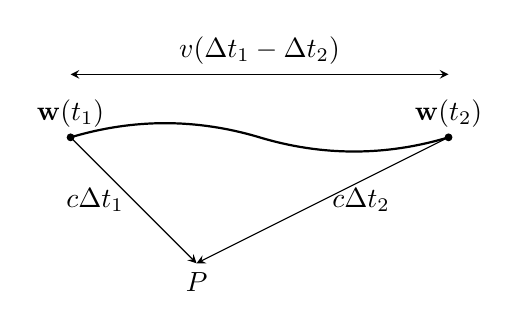
\begin{tikzpicture}[scale=0.8]

	  % Wiggly/smooth path between two nodes
	  \draw[thick] 
		(-3,0) .. controls (-2,0.3) and (-1,0.3) .. (0,0)
			   .. controls (1,-0.3) and (2,-0.3) .. (3,0);

	  % Endpoints (optional)
	  \filldraw (-3,0) circle (1.5pt) node[above] {\( \mathbf{w}(t_1) \)};
	  \filldraw (3,0) circle (1.5pt) node[above] {\( \mathbf{w}(t_2) \)};


	  \draw[-stealth] (-3, 0) -- node[midway, left] {\( c \Delta t_1 \)} (-1, -2);
	  \draw[-stealth] (3, 0) -- node[midway, right] {\( c \Delta t_2 \)} (-1, -2);
	  \node at (-1, -2.3) {\( P \)};

	  \draw[stealth-stealth] (-3, 1) -- node[midway, above] {\( v(\Delta t_1 - \Delta t_2) \)} (3, 1);
	\end{tikzpicture}	
\end{center}
If this were true, then by the triangle inequality, we'd be able to write:
\begin{align*}
	v(\Delta t_1 - \Delta t_2) + c \Delta t_2 &\geq c \Delta t_1\\
	v(\Delta t_1 - \Delta t_2) &\geq c(\Delta t_1 - \Delta t_2)\\
	\therefore v &\geq c
\end{align*}
so if this were true, we are forced to conclude that the particle travels faster than the speed of light,
which is impossible for massive particles (that is, particles having mass). 

Now, one final comment before we end today's lecture. The discussion so far with the potentials is only true
for point sources. But, now consider sources which are distributed over a non-point volume. 
Due to the retarded time, the volume we integrate over to calculate \( V(t, \mathbf{r}) \), even though we
integrate at a fixed time, is not going to be the volume over which the charge is distributed. To illustrate
this further, consider the following scenario:
\begin{center}
	\begin{tikzpicture}[decoration = snake]
 
	\node[cylinder, 
		draw = black, 
		minimum width = 1cm,
		minimum height = 2.5cm] (c) at (0,0) {};

	\node[cylinder, 
		draw = green!80!white, 
		dashed,
		minimum width = 1cm,
		minimum height = 2.5cm] (c) at (-1,0) {};

	\draw[decorate, -stealth, red!80!white] (1.2, 0) -- (1.9, 0);
	\draw[decorate, -stealth, green!80!white] (-2.1, 0) -- (-1.4, 0);
	\filldraw (4, 0) circle (1.5pt) node[right] {\( P \)};
\end{tikzpicture}
\end{center}
Suppose we want to evaluate the field at \( P \). The contribution from the front of the cylinder (red) takes a
certain time to arrive, but the back (green) takes a \textit{longer} time to cover that same distance. Therefore, the
signal measured at time \( t \) comes from the contribution of the front, and also the back but at an earlier
point in time, to compensate for that extra travel distance. So, when we integrate over the entire volume, we
aren't integrating over the charge distribution, but an extended version of the charge distribution to
account for the time of travel. We will continue this discussion next lecture.





